% Based on docs/ambiguities/template.tex. Build: make questions LECTURE=10
\documentclass[a4paper,12pt]{article}
\usepackage[margin=19mm]{geometry}
\usepackage{amsmath,amssymb,graphicx,xcolor}
\usepackage{fontspec}
\usepackage{xepersian}
\settextfont{XB Roya}
\setlatintextfont{Latin Modern Roman}
\definecolor{ink}{HTML}{173D75}
\graphicspath{{images/}}
\setlength{\parindent}{0pt}
\setlength{\parskip}{5pt}
\linespread{1.08}
\newcommand{\qtitle}[2]{{\Large\bfseries\color{ink} پرسش \lr{#1}: #2}\par}
\newcommand{\answer}{\medskip\textbf{پاسخ یا صورت مورد تأیید و تاریخ:}\par\vspace{16mm}\hrule\medskip}
\newcommand{\sourcefile}{\begin{LTR}\footnotesize\texttt{sources/lectures/10 Notherian and Artinian modules.pdf}\end{LTR}}
\begin{document}
{\LARGE\bfseries پرسش‌های ابهام جلسهٔ ۱۰}\par
جزوهٔ جبر پیشرفتهٔ دکتر خسروی؛ بازبینی \lr{2026-10-25}.\par
شماره‌ها، صفحهٔ یک‌مبنای فایل پی‌دی‌اف‌اند.
پرسش‌های زیر هنوز پاسخ ندارند و اصلاح‌های پیشنهادی، متن قطعی اسلایدها نیستند.
\medskip\hrule\medskip

\qtitle{L10-Q01}{فرض ناصفر بودن حلقه}
\textbf{وضعیت:} در انتظار پاسخ؛ پاسخ و تصمیمی ثبت نشده است.
\textbf{نشانی منبع:} نسخهٔ \lr{primary}، صفحهٔ ۲، قضیهٔ پایین صفحه؛ صفحهٔ ۳، پایان برهان دترمینانی.
\sourcefile
\begin{center}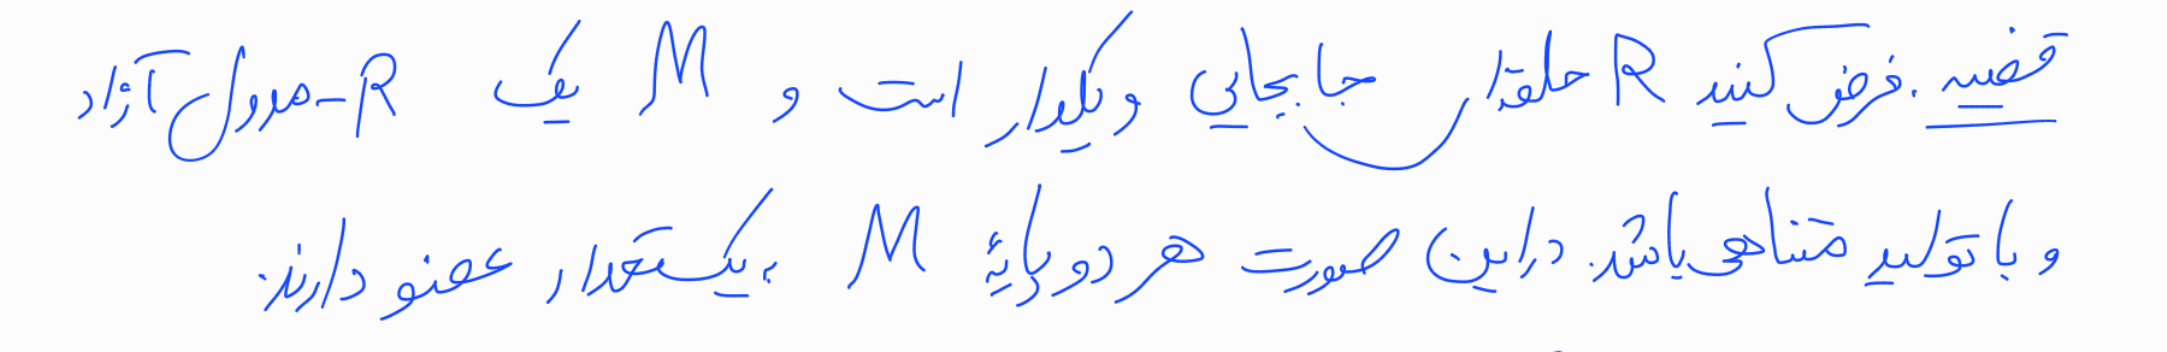
\includegraphics[width=\linewidth,height=34mm,keepaspectratio]{L10-Q01-hypotheses.png}\end{center}
\textbf{عبارت منبع:} حلقهٔ $R$ «جابجایی و یکدار» فرض شده است؛ برهان با $0=1$ به تناقض می‌رسد.
\begin{center}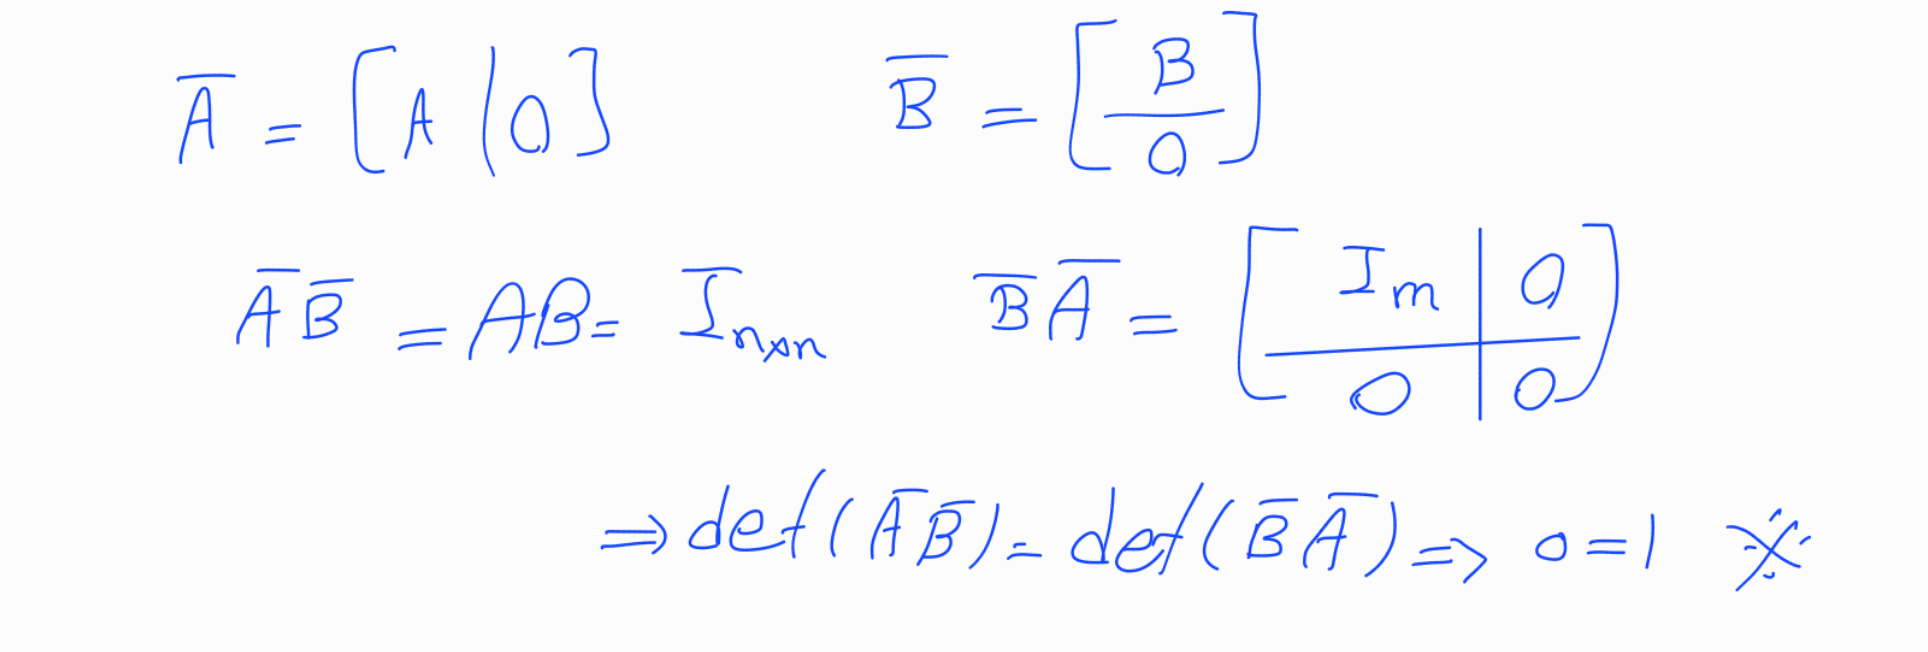
\includegraphics[width=\linewidth,height=49mm,keepaspectratio]{L10-Q01-determinants.png}\end{center}
\textbf{خوانش‌ها و اثر تفاوت:} ممکن است $1_R\ne0_R$ از قرارداد درس منظور باشد، یا لازم باشد این فرض به قضیه افزوده شود. با مجاز بودن حلقهٔ صفر، $0=1$ تناقض نیست و استدلال برابری تعداد اعضای دو پایه به این صورت کافی نیست.
\textbf{پرسش:} آیا در این قضیه $R$ ناصفر است؟ اگر بله، این قید را صریحاً در صورت اسلاید درج کنیم؟
\answer

\newpage
\qtitle{L10-Q02}{زیرگروه‌های پروفر و توان مخرج}
\textbf{وضعیت:} در انتظار پاسخ؛ پاسخ و تصمیمی ثبت نشده است.
\textbf{نشانی منبع:} نسخهٔ \lr{primary}، صفحهٔ ۵، ادعای چهارم در پایین صفحه؛ صفحهٔ ۶، دو حالت برهان و نتیجه.
\sourcefile
\begin{center}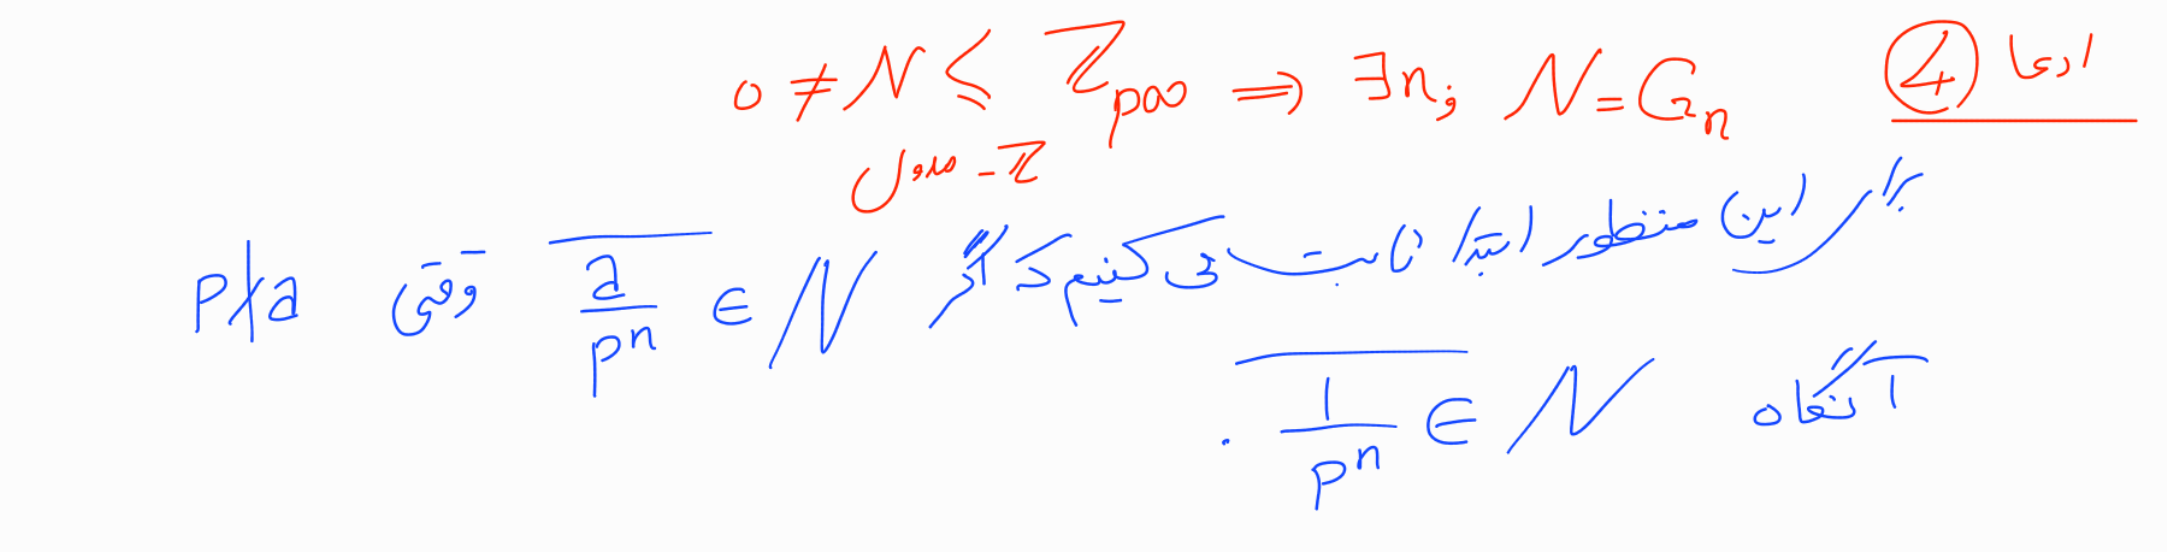
\includegraphics[width=\linewidth,height=38mm,keepaspectratio]{L10-Q02-claim.png}\end{center}
\textbf{عبارت منبع:}
\[
 0\ne N\leq\mathbb Z_{p^\infty}\ \Longrightarrow\ \exists n:\ N=G_n.
\]
ولی در صفحهٔ بعد، حالت نبودن بزرگ‌ترین توان مخرج به $N=\mathbb Z_{p^\infty}$ می‌انجامد:
\begin{center}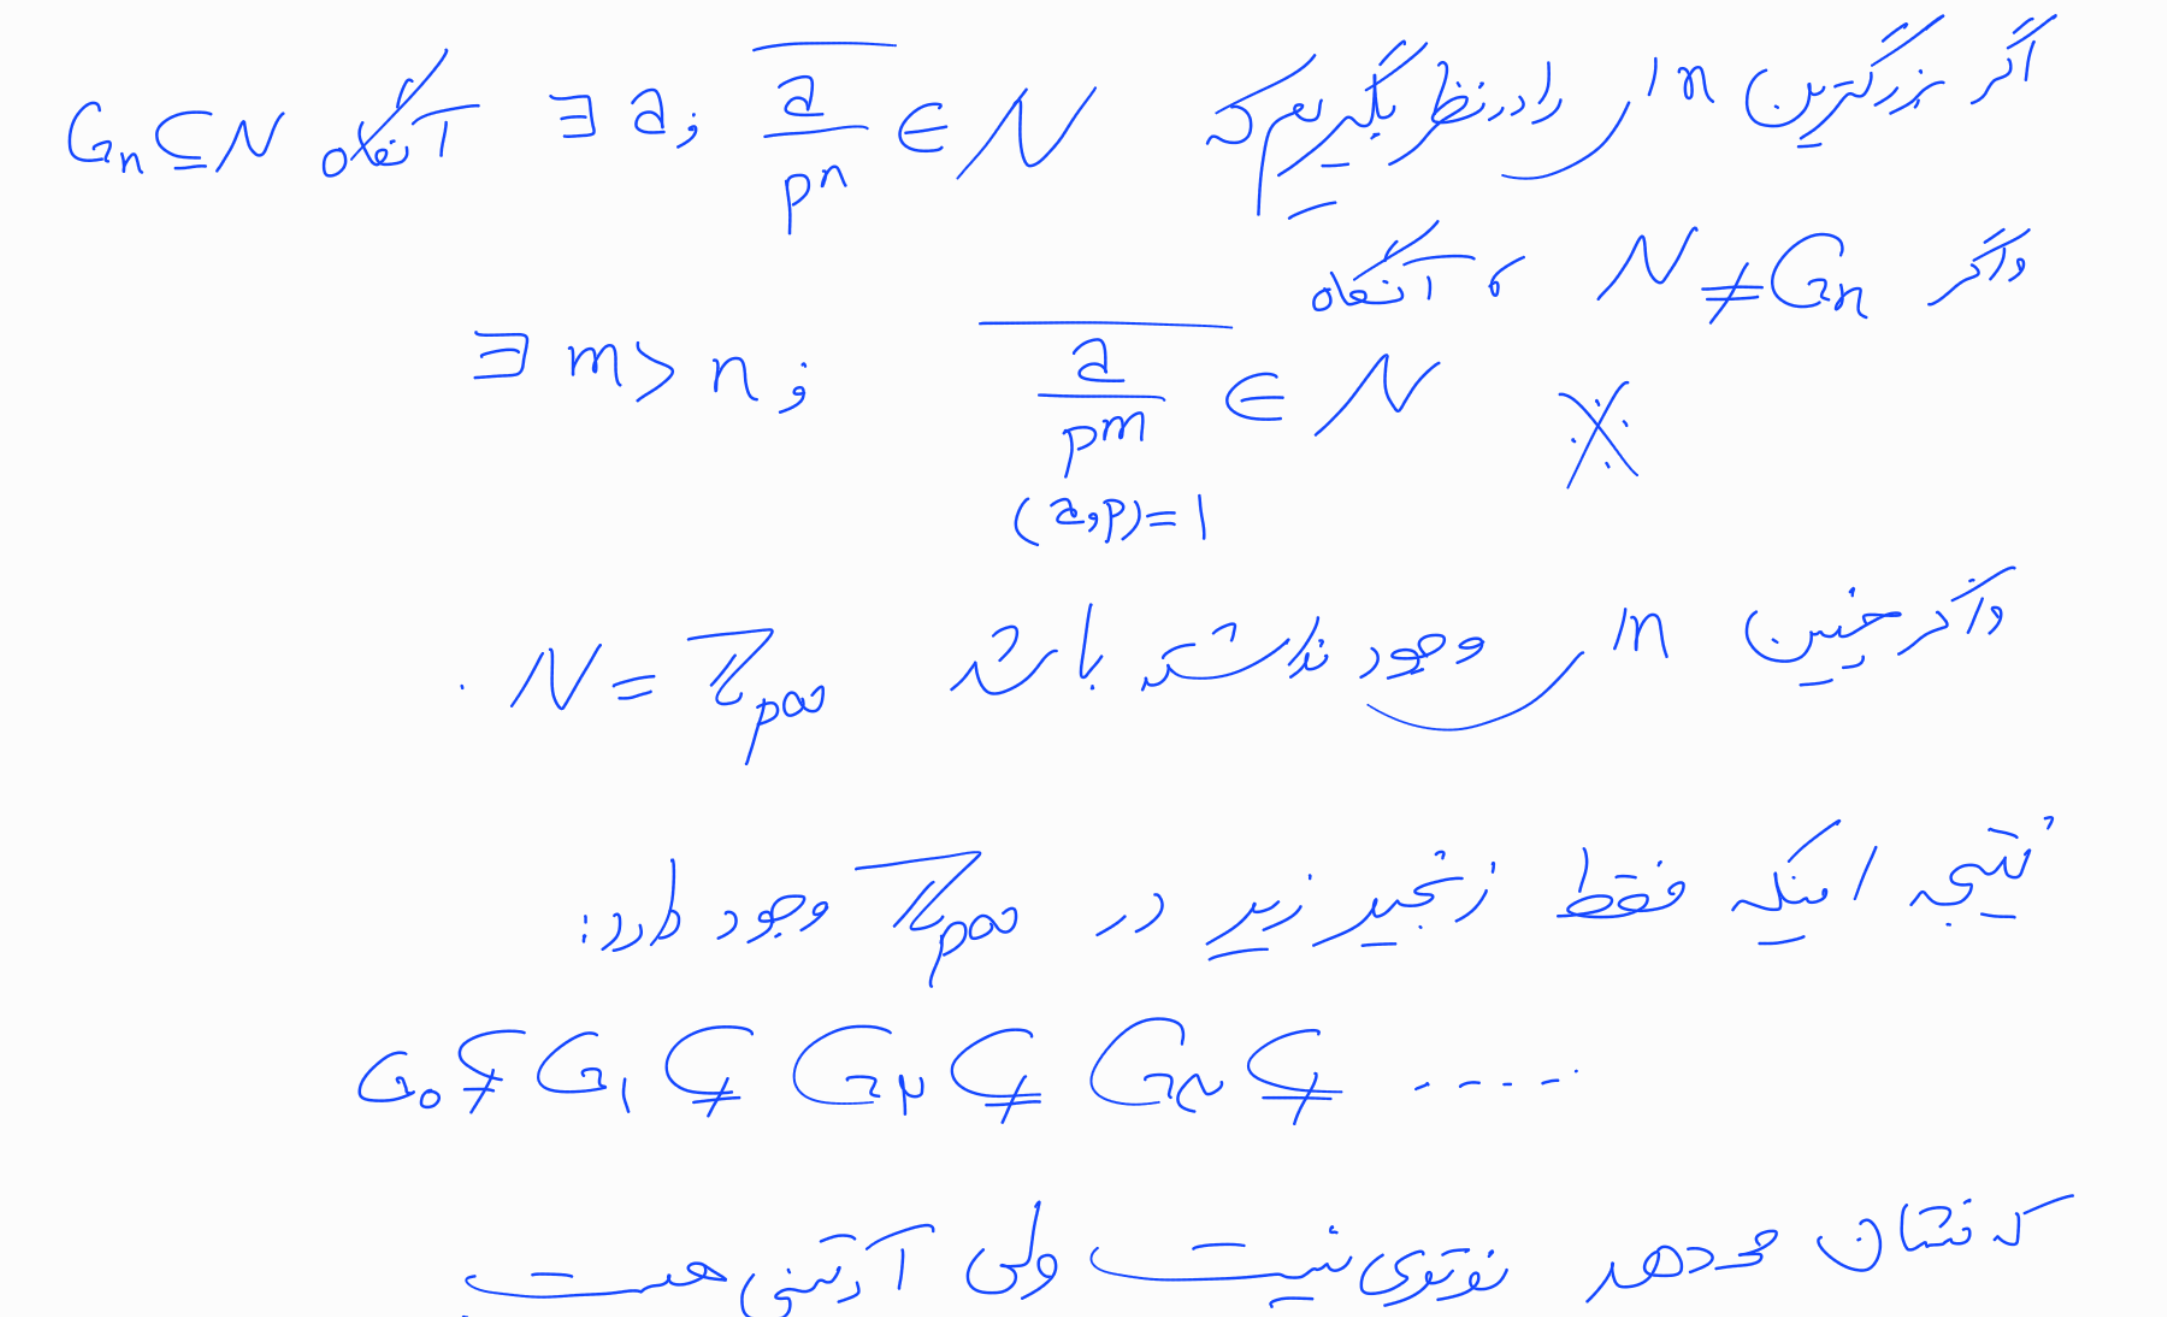
\includegraphics[width=\linewidth,height=60mm,keepaspectratio]{L10-Q02-cases.png}\end{center}
\textbf{خوانش‌ها و اثر تفاوت:} ادعای چهارم با $\leq$ شامل کل گروه می‌شود، در حالی که حالت دوم آن را جدا می‌کند. همچنین عبارت «بزرگ‌ترین $n$» اگر بر همهٔ نمایش‌های $\overline{a/p^n}$ اعمال شود، به‌علت امکان ضرب صورت و مخرج در $p$ معنای مورد نیاز را ندارد.
\textbf{پرسش:} آیا منظور این است که هر زیرگروه ناصفرِ \textbf{سره} برابر یک $G_n$ است و کل گروه حالت جداگانه است؟ در برهان نیز بزرگ‌ترین توان مخرج را فقط برای نمایش‌های تحویل‌یافته با $p\nmid a$ بگیریم؟
\answer

\newpage
\qtitle{L10-Q03}{اندیس توقف در برهان شرط ماکسیمال}
\textbf{وضعیت:} در انتظار پاسخ؛ پاسخ و تصمیمی ثبت نشده است.
\textbf{نشانی منبع:} نسخهٔ \lr{primary}، صفحهٔ ۷، چهار سطر پایانی برهانِ گذار از تولید متناهی به وجود عضو ماکسیمال.
\sourcefile
\begin{center}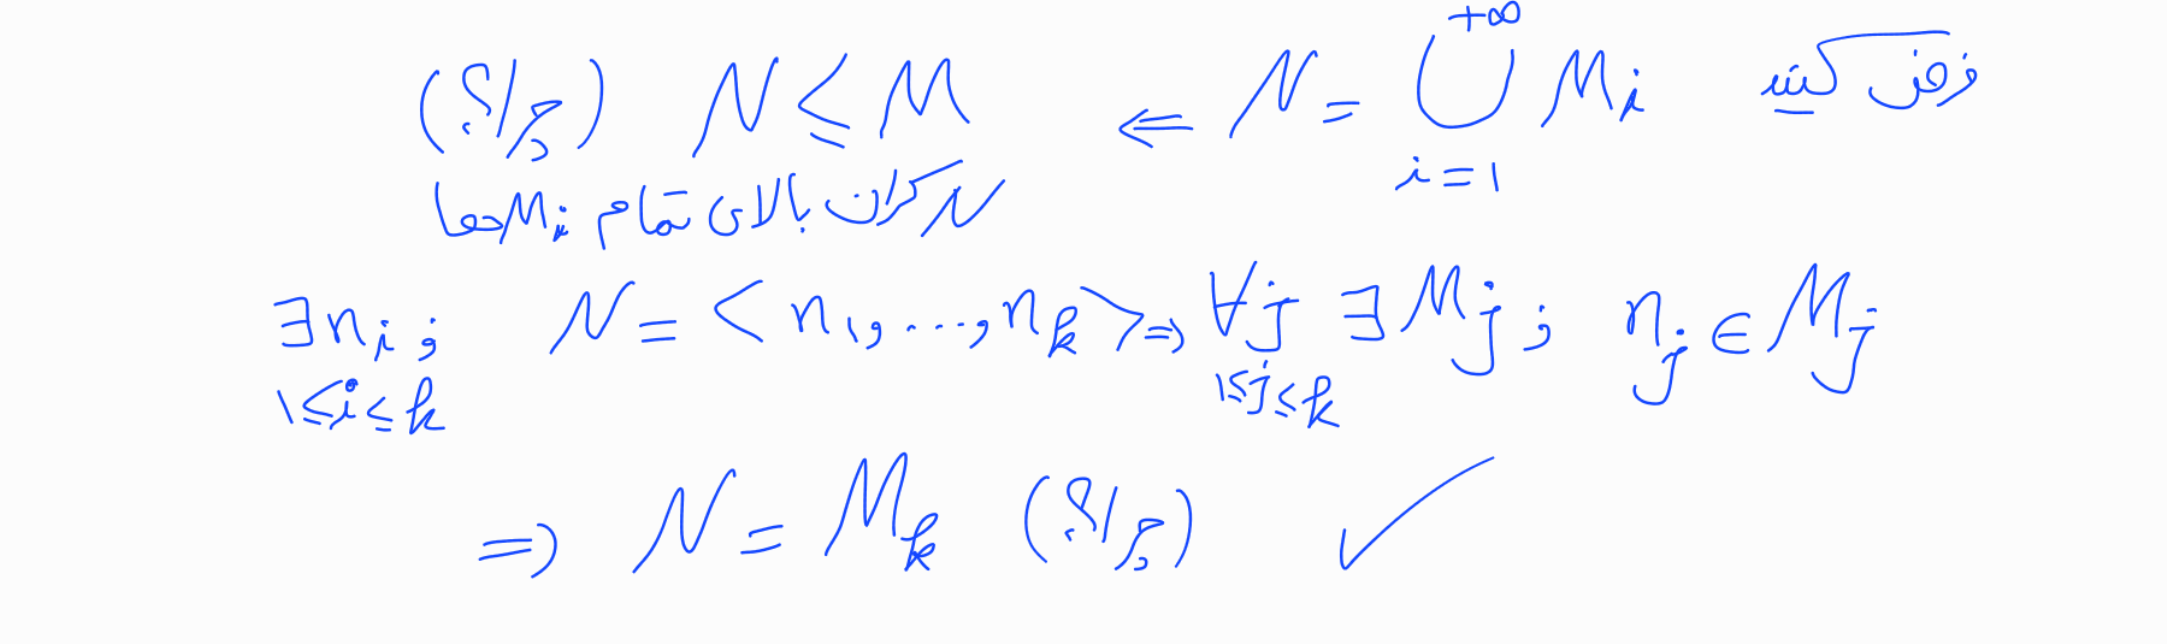
\includegraphics[width=\linewidth,height=62mm,keepaspectratio]{L10-Q03-index.png}\end{center}
\textbf{عبارت منبع:} برای زنجیر اکید $M_1\subsetneq M_2\subsetneq\cdots$ نوشته شده است:
\[
 N=\bigcup_{i=1}^{\infty}M_i=\langle n_1,\ldots,n_k\rangle,
 \qquad N=M_k.
\]
برای هر مولد، عضویت در یکی از زیرمدول‌های زنجیر ذکر شده، ولی اندیسی که همهٔ مولدها را در بر گیرد صریحاً تعریف نشده است.
\textbf{خوانش‌ها و اثر تفاوت:} ممکن است $k$ در سطر آخر صرفاً نام تازه‌ای برای یک اندیس به‌اندازهٔ کافی بزرگ باشد؛ اگر همان تعداد مولدها باشد، $N=M_k$ از مقدمات نوشته‌شده به دست نمی‌آید.
\textbf{صورت پیشنهادی برای تأیید:}
\[
 n_i\in M_{j_i}\ (1\leq i\leq k),\qquad
 K=\max\{j_1,\ldots,j_k\},\qquad N=M_K.
\]
آنگاه $M_{K+1}\subseteq N=M_K$ با اکید بودن زنجیر تناقض دارد.
\textbf{پرسش:} آیا همین انتخاب $K$ و تناقضِ سطر بعد، تکمیل مورد نظر جزوه است؟ آن را با اندیس مستقل $K$ در اسلاید بنویسیم؟
\answer
\end{document}
